\documentclass{beamer}
\usepackage[utf8]{inputenc}
\usepackage{hyperref}
\usepackage{amsmath,amsfonts,amsthm,bm}
\usepackage{color}
\usepackage{minted}
\usepackage{graphicx}
\usepackage{booktabs}
\usepackage{tikz}
\usepackage{pgfplots}

\hypersetup{
    colorlinks=true,
    linkcolor=red,
    filecolor=magenta,      
    urlcolor=red,
}

\DeclareMathOperator*{\argmax}{argmax}
\DeclareMathOperator*{\argmin}{argmin}
\let \vec \mathbf

\mode<presentation> {
    \usetheme{CambridgeUS}
    \setbeamertemplate{footline}[page number]
    \setbeamertemplate{navigation symbols}{}
}


\title[Linear Methods]{Linear Methods}

\author{Shyue Ping Ong}
\institute[UCSD]{University of California, San Diego\\
\medskip
}
\date{NANO281}

\begin{document}


\begin{frame}
    \titlepage % Print the title page as the first slide
\end{frame}


\begin{frame}{Overview}
    \tableofcontents
\end{frame}


\section{Preliminaries}

\begin{frame}{Preliminaries}
    \begin{itemize}
        \item We will go very deep into linear models.
        \item Most of you probably have seen linear models in some form, but we will start from scratch to further illustrate key concepts such as bias and variance.
        \item We will then discuss techniques such as regularization and transformation of inputs in the context of linear methods.
    \end{itemize}
\end{frame}

\begin{frame}{Notation}
    \begin{itemize}
        \item Capital letters, e.g., $X$ denote variables.
        \item Lower-case letters e.g., $x$, denote observations.
        \item Dummy index $j$ to denotes different variables, e.g., $X_j$
        \item Dummy index $i$ to denotes different observations, e.g., $x_i$
        \item Bolded variables are vector/matrices, e.g., $\vec{y}$, $\vec{X}$
    \end{itemize}
\end{frame}

\section{Linear regression}

\begin{frame}{Linear Regression}
    \Huge{\centerline{Linear Regression}}
\end{frame} 

\begin{frame}{Simplest possible model between target and feature}
    \begin{equation*}
        Y=f(X_1,X_2,...,X_p)= \beta_0 + \sum_{j=1}^p \beta_j X_j
    \end{equation*}
    $X_j$ can be:
    \begin{itemize}
        \item Quantitative inputs
        \item Transformations of quantitative inputs, e.g., log, exp, powers, etc.
        Basis expansions, e.g., $X_2 = X_1^2$, $X_3 = X_1^3$
        \item Interactions between variables
        \item Encoding of levels of inputs
    \end{itemize}
\end{frame}


\begin{frame}{Supervised learning}
    \begin{itemize}
        \item Given a set of paired observations $\{x_{ij}, y_i\}$, what are the model parameters (in this case, the coefficients $\beta_j$) that are ``optimal''?
        \item ``Optimal'' is typically defined as minimization of some \textbf{loss function} (also known as \textbf{cost function}) that measures the error of the model.
    \end{itemize}
\end{frame}


\begin{frame}{Least squares regression}
    Consider the simple case of
    \begin{equation*}
        Y = \beta_0 + \beta_1 X_1
    \end{equation*}
    In least squares regression, the loss function is defined as the sum squared error given the $N$ observations:
    \begin{eqnarray*}
        L(Y, \hat{f}(X)) & = & \sum_{i=1}^N (y_i - f(x_i))^2 \\
        & = & \sum_{i=1}^N (y_i - \beta_0 - \beta_1 x_{i1})^2
    \end{eqnarray*}
    \end{frame}

    \begin{frame}{What are the optimal parameters $\beta_0$ and $\beta_1$?}
       \Huge{\centerline{Derivation in class...}}
    \end{frame}

    \begin{frame}{Reformulating the general multiple linear regression as a vector equation…}
    Considering $N$ observations of
    \begin{equation*}
        y_i = \beta_0 + \beta_1 x_{i1} + + \beta_2 x_{i2} + ... + \beta_p x_{ip}
    \end{equation*}
    Let
    \begin{equation*}
        \vec{y} = \begin{pmatrix}y_1\\y_2\\...\\y_n\end{pmatrix}, \bm{\beta} = \begin{pmatrix}\beta_0\\\beta_1\\...\\\beta_p\end{pmatrix}, \vec{X} = \begin{pmatrix}1 & x_{11} & x_{12} & ... & x_{1p}\\
        1 & x_{21} & x_{22} & ... & x_{2p}\\
        \vdots & & & & \\
        1 & x_{N1} & x_{N2} & ... & x_{Np}\end{pmatrix}, 
    \end{equation*}
    So, 
    \begin{equation*}
        \vec{y} = \vec{X}\bm{\beta} 
    \end{equation*}
    Note that $\vec{y}$ is a $N \times 1$ vector,
    $\bm{\beta}$ is a $(p+1) \times 1$ vector, and $\vec{X}$ is a  $N \times (p+1)$ matrix.
\end{frame}


\begin{frame}{Reformulating the general multiple linear regression as a vector equation…}
    \begin{equation*}
        L = RSS = (\vec{y} - \vec{X}\bm{\beta})^T(\vec{y} - \vec{X}\bm{\beta})
    \end{equation*}
    Assuming (for the moment) that $\vec{X}$ has full column rank, and hence $\vec{X}^T\vec{X}$ is positive definite, It can be shown using the same principles that the following unique solution for $\bm{\beta}$ is:
    \begin{eqnarray*}
        \hat{\bm{\beta}} &=& (\vec{X}^T \vec{X})^{-1} \vec{X}^T \vec{y} \\
        \hat{\vec{y}} & = & \vec{X} \hat{\bm{\beta}} = \vec{X}(\vec{X}^T \vec{X})^{-1} \vec{X}^T \vec{y} 
    \end{eqnarray*}
\end{frame}


\begin{frame}{Graphic representation of MLR with two dependent variables}
    \begin{figure}
        \centering
        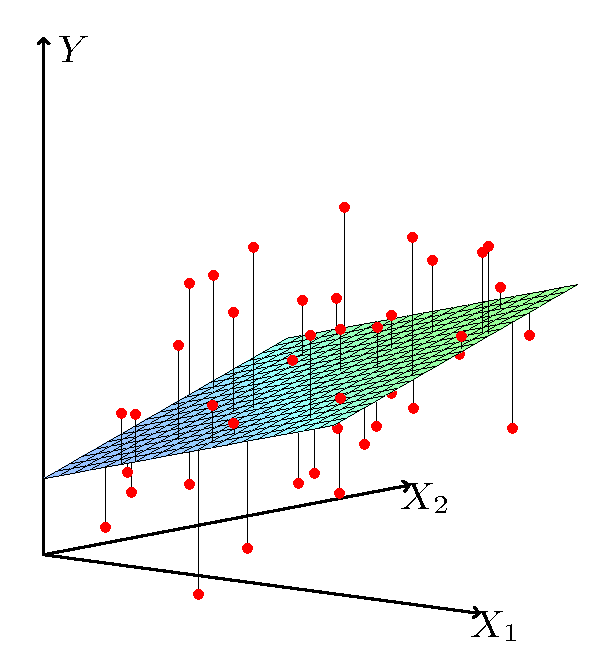
\includegraphics[width=0.35\textwidth]{figures/fig3-1.pdf}
        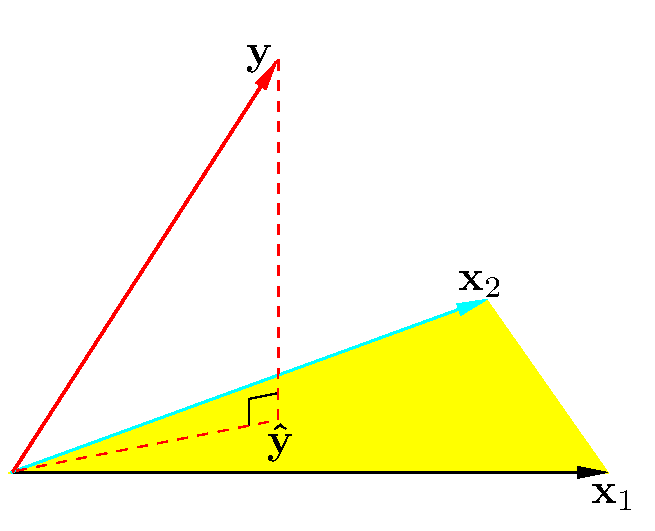
\includegraphics[width=0.35\textwidth]{figures/fig3-2.pdf}
        \caption{MLR minimizes sum square of residuals. The projection $\vec{\hat{y}}$ represents the vector of the least squares predictions onto the hyperplane spanned by the input vectors $\vec{x_1}$ and $\vec{x_2}$. \cite{hastieElementsStatisticalLearning2016}.}
    \end{figure}
\end{frame}


\begin{frame}{Validity of least squares criterion}
    \begin{itemize}
        \item Observations are independently drawn at random.
        \item Variance of $\vec{y}$ is constant given by $\sigma^2$.
    \begin{equation*}
        \mathrm{var}(\hat{\bm{\beta}}) = (\vec{X}^T \vec{X})^{-1} \sigma^2
    \end{equation*}
    \item and $\sigma$ is estimated using:
    \begin{equation*}
        \sigma^2 = \frac{1}{N-p-1}\sum_{i=1}^N (y_i - \hat{y_i})^2
    \end{equation*}
    \end{itemize}
\end{frame}


\begin{frame}{Hypothesis Testing for Coefficients}
    \begin{itemize}
        \item To derive insights into a model, we often want to know which of the input parameters are the most relevant to the target.
        \item Under assumptions of the errors in $y$ follow a Gaussian distribution $N(0, \sigma^2)$, the errors in $\hat{\bm{\beta}}$ also have a Gaussian distribution $N(\beta, (\vec{X}^T \vec{X})^{-1} \sigma^2)$
        \item Hypothesis testing can be carried out for whether a particular $\beta_j$ is 0 using the following test statistic:
        \begin{equation*}
        t_j = \frac{\hat{\bm{\beta_j}}}{\sigma\sqrt{v_j}}
        \end{equation*}
        where $v_j$ is the $j$th diagonal element of $(\vec{X}^T \vec{X})^{-1}$. $t_j$ has a $t$ distribution with $N-p-1$ degrees of freedom (dof).
    \end{itemize}
\end{frame} 


\begin{frame}{Hypothesis Testing for Groups of Coefficients}
    \begin{itemize}
        \item More often, we want to test groups of coefficient for significance. E.g., to the $k$ levels of a categorical variable.
        \item We will use the following $F$ statistic:
        \begin{equation*}
        F = \frac{(\mathrm{RSS}_0 - \mathrm{RSS}_1)/(p_1-p_0)}{\mathrm{RSS}_1/(N-p_1-1)}
        \end{equation*}
        where $\mathrm{RSS}_0$ is the RSS of the larger model with $p_0 + 1$ parameters and $\mathrm{RSS}_1$ is the RSS of the smaller model with $p_1 + 1$ parameters with $p_0 - p_1$ parameters set to zero. The $F$ statistic has a distribution of $F_{p_1-p_0,N-p_1-1}$.
    \end{itemize}
\end{frame} 


\begin{frame}{Gauss-Markov Theorem}
    \begin{itemize}
        \item Consider the estimator $\hat{\theta}$ for a variable $\theta$.
        \begin{eqnarray*}
            \mathrm{MSE} & = & E(\hat{\theta} - \theta)^2 \\
            & = & \mathrm{var}(\hat{\theta}) + [E(\hat{\theta}) - \theta]^2
        \end{eqnarray*}
        \item The MSE can be broken down into the variance of the estimate itself and the square of the bias.
        \begin{block}{Gauss-Markov Theorem}
        The least squares estimator has the smallest variance among all linear \textit{unbiased} estimators.
        \end{block}
        \item However, there can be estimators that are biased with smaller MSE.
    \end{itemize}
\end{frame}


\begin{frame}{Example materials data}
    \begin{columns}
    \begin{column}{0.6\textwidth}
        \begin{itemize}
            \item Target: Bulk modulus of elements (from Materials Project)
            \item Candidate features:
            \begin{itemize}
                \item Melting point (MP)
                \item Boiling point (MP)
                \item Atomic number (Z)
                \item Electronegativity ($\chi$)
                \item Atomic radius ($r$)
            \end{itemize}
            \item Question: Why these features?
            \item We will add some transformations of these inputs as well, i.e., the square and square root of the electronegativity and atomic radius.
    \end{itemize}
    \end{column}
    \begin{column}{0.4\textwidth}
        \begin{figure}
        \centering
        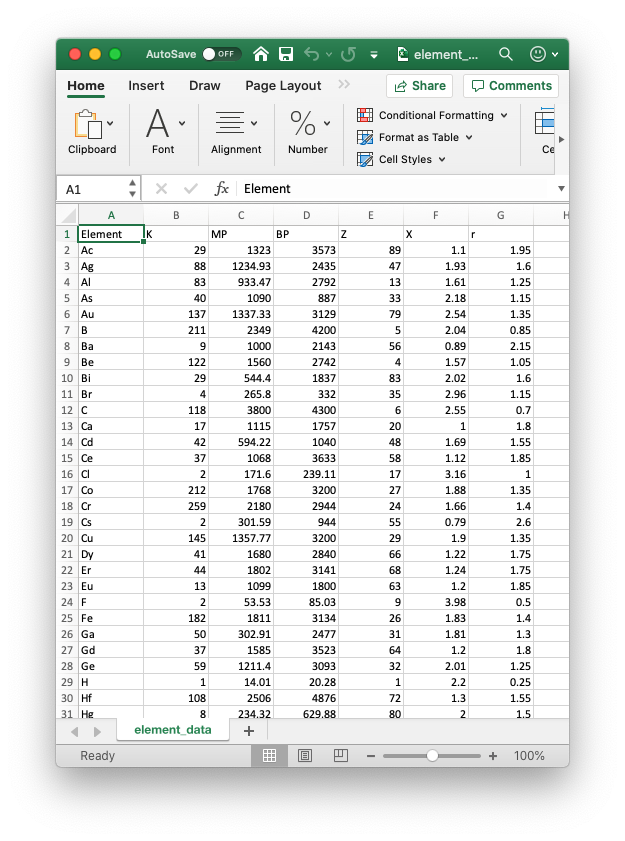
\includegraphics[width=\textwidth]{figures/elementdata.png}
    \end{figure}
    \end{column}
\end{columns}
\end{frame} 


\begin{frame}[fragile]{Using pandas for easy data manipulation}
    \begin{minted}{python}
import pandas as pd
# Read in data and set first column as index.
data = pd.read_csv("element_data.csv", index_col=0)
# Generate transformations as additional columns.
data["X^2"] = data["X"] ** 2
data["sqrt(X)"] = data["X"] ** 0.5
data["r^2"] = data["r"] ** 2
data["sqrt(r)"] = data["r"] ** 0.5
# Define our features, which is all the columns
# excluding K, which is the target.
features = [c for c in data.columns if c != "K"]
x = data[features]
y = data["K"]
\end{minted}

Recommendation: Go through the \href{https://pandas.pydata.org/pandas-docs/stable/getting_started/10min.html}{10 minute guide to pandas}.
\end{frame} 


\begin{frame}[fragile]{MLR in scikit-learn}
\begin{minted}{python}
from sklearn import linear_model
reg = linear_model.LinearRegression()
reg.fit(x, y)
print(ref.coef_)
print(reg.intercept_)
\end{minted}

\begin{itemize}
    \item Note that x should contain the features only - there is no need to add a 1 column for the intercept. By default, the parameter fit\_intercept in sklearn.linear\_model.LinearRegression is True. You can set it to False to do a MLR without intercept.
    \item Documentation: \href{https://scikit-learn.org/stable/modules/generated/sklearn.linear_model.LinearRegression.html}{link}.
\end{itemize}

\end{frame} 


\section{Model selection}

\begin{frame}{Model selection}
    \Huge{\centerline{Model selection}}
\end{frame} 


\begin{frame}{Model performance}
    \begin{itemize}
        \item We will take a brief digression into model assessment and selection before continuing on to other linear methods.
        \item Model performance is related to its performance on \textit{independent test data}, i.e., one cannot simply report a model's performance on training data alone.
        \item Note that this section is deliberately limited to high level concepts that are needed to continue further in exploration of linear methods. A more detailed discussion will be performed in later lectures.
    \end{itemize}
\end{frame} 


\begin{frame}{Typical measures of model performance}
    \begin{itemize}
        \item Mean squared error (MSE):
            \begin{equation*}
                L(Y, \hat{f}(X)) = \frac{1}{N}\sum_{i=1}^N (y_i - f(x_i))^2
            \end{equation*}
        \item Mean absolute error (MAE):
            \begin{equation*}
                L(Y, \hat{f}(X)) = \frac{1}{N}\sum_{i=1}^N \left| y_i - f(x_i) \right|
            \end{equation*}
        \item Test error: $L$ over independent test set.
        \item Training error: $L$ over training set.
    \end{itemize}
\end{frame}


\begin{frame}{Training and test errors with model complexity}
    \begin{itemize}
        \item Model complexity increases as the number of parameters increases (e.g., number of independent variables in MLR). 
        \item Training errors \textbf{always} decrease with increasing model complexity.
        \item However, test errors do not have a monotonic relationship with model complexity. Test errors are high when model complexity is too low (underfitting) or too high (overfitting).
    \end{itemize}
    \begin{figure}
        \centering
        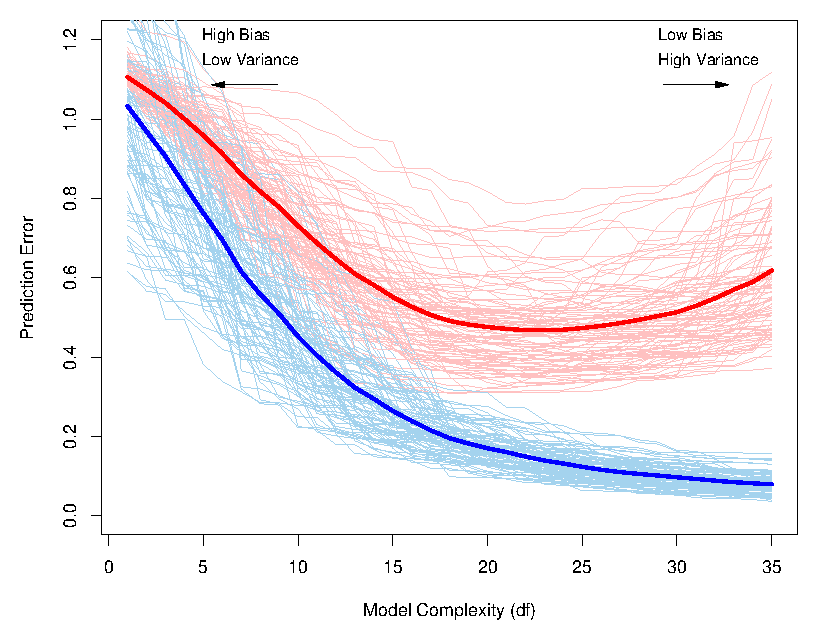
\includegraphics[width=0.5\textwidth]{figures/fig7-1.pdf}
    \end{figure}
\end{frame}


\begin{frame}{Training, validation and test data}
    \begin{itemize}
        \item Model selection: estimating the performance of different models in order to choose the best one.
        \item Model assessment: having chosen a final model, estimating its prediction error (generalization error) on new data.
        \item Ideal data-rich situation: Divide data into three parts:
        \begin{itemize}
            \item Training set: For training the model.
            \item Validation set: For estimating prediction error to select the model.
            \item Test set: For assessing the generalization error of the final model.
        \end{itemize}
        \item Typical training:validation:test split is 50:25:25 or 80:10:10, or in very data-poor situations, maybe even 90:5:5.
        \item Note that at no point in the model fitting process should the test set be ``seen''.
    \end{itemize}
\end{frame}


\begin{frame}{$K$-fold cross validation (CV)}
    \begin{itemize}
        \item Simplest and most widely used approach for model validation.
        \item Data set is split into $K$ buckets (usually by random).
        \item Typical values of $K$ is 5 or 10. $K = N$ is known as ``leave-one-out'' CV.
        \begin{table}
        \begin{tabular}{|p{1.7cm}|p{1.7cm}|p{1.7cm}|p{1.7cm}|p{1.7cm}|}
            \hline
            \Large{Train} & \Large{Train} & \textcolor{red}{\Large{Validate}} & \Large{Train} & \Large{Train}\\
            \hline
        \end{tabular}
        \end{table}
        \item CV score is computed on the validate data set after training on the train data:
        \begin{equation*}
                CV(\hat{f}^{-k(i)},\alpha) = \frac{1}{N_{k(i)}}\sum_{i=1}^{N_{k(i)}} L(y_i, \hat{f}^{-k(i)}(x_i,\alpha))
        \end{equation*}
        \item assuming the $k^{th}$ data bucket has $N_{k(i)}$ data points and $\hat{f}^{-k(i)}$ refers to the model fitted with the $k^{th}$ data left out ($N-N_{k(i)}$ data in fitting).
    \end{itemize}
\end{frame}


\begin{frame}[fragile]{CV in scikit-learn}
\begin{minted}{python}
from sklearn.model_selection import cross_validate, KFold
kfold = KFold(n_splits=5, shuffle=True, random_state=42)
cv_results = cross_validate(ridge, z, y, cv=kfold)
\end{minted}
\begin{itemize}
    \item Note that we have customized the KFold object passed to the cross\_validate method. The reason is that our element data is non-random by default. So we want to perform shuffling prior to doing the splits.
    \item Documentation: \href{https://scikit-learn.org/stable/modules/generated/sklearn.model_selection.cross_validate.html?highlight=cross_validate#sklearn.model_selection.cross_validate}{link}.
\end{itemize}
\end{frame}


\begin{frame}{Characteristics of the example materials dataset}
    \begin{itemize}
        \item Before proceeding further, let us try to tease out some aspects of the dataset.
        \item Quite clearly, there are correlations between some sets of variables.
        \item In other words, the input features are \textbf{non-orthonormal} with each other.
        \begin{figure}
            \centering
            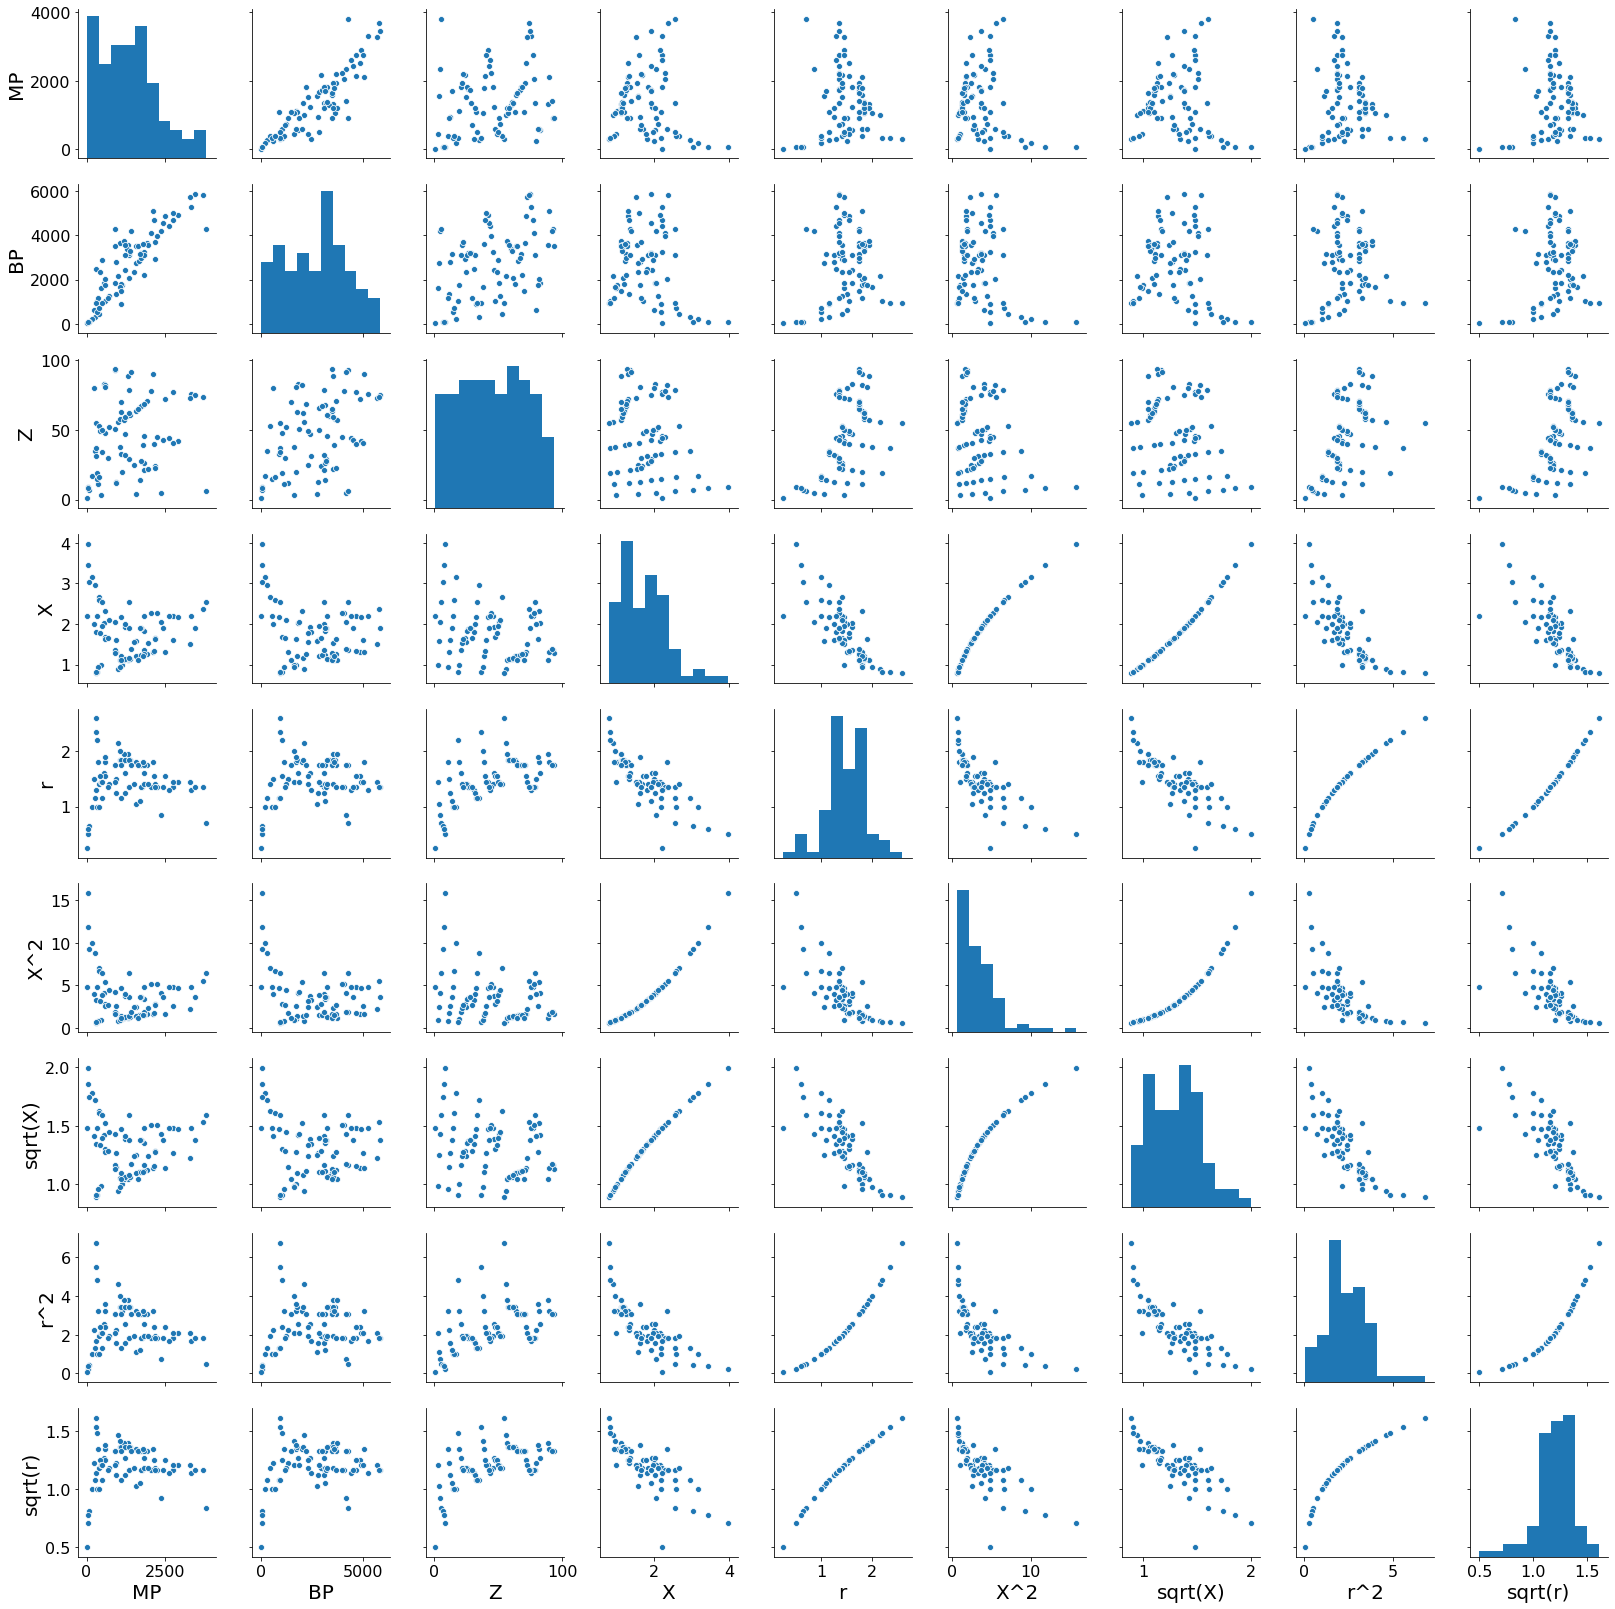
\includegraphics[width=0.45\textwidth]{figures/pairplot-materialsdata.png}
            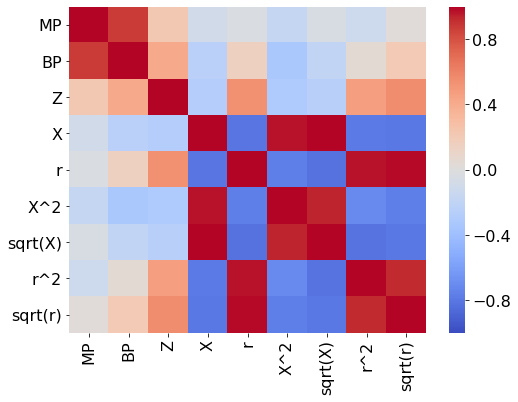
\includegraphics[width=0.45\textwidth]{figures/paircorrelations-materialsdata.png}
        \end{figure}
    \end{itemize}
\end{frame}


\begin{frame}{Demo}
    \centerline{\href{https://github.com/materialsvirtuallab/nano281/tree/master/lectures}{Notebook}}
    \centerline{\href{https://mybinder.org/v2/gh/materialsvirtuallab/nano281/master?filepath=lectures}{Binder}}
\end{frame} 


\section{Beyond least squares}


\begin{frame}{Beyond least squares}
    \Huge{\centerline{Beyond least squares}}
\end{frame} 

\begin{frame}{Model selection}
    \begin{itemize}
        \item Often, we want to improve on the least squares model.
        \begin{itemize}
            \item To improve prediction accuracy by sacrificing some bias for reduced variance.
            \item To improve interpretability by reducing number of features or descriptors.
        \end{itemize}
        \item Three main approaches:
        \begin{enumerate}
            \item Subset selection
            \item Shrinkage methods
            \item Dimension reduction
        \end{enumerate}
    \end{itemize}
\end{frame}


\subsection{Subset selection}

\begin{frame}{Subset selection}
    Best subset selection
    \begin{itemize}
        \item Brute force approach.
        \item From $p$ parameters, find the subset of $k$ parameters that results in the smallest RSS.
        \item Combinatorially expensive for large $p$ and large $k$.
        \item Note that the best subset for a larger $k$ does not necessarily include the best subset for a smaller $k$.
    \end{itemize}
    Forward- or backward-stepwise selection
    \begin{itemize}
        \item Forward: Start with intercept, and iteratively add feature that most improves the fit.
        \item Backward: Start with full model, and sequentially deletes the feature with least impact on the fit.
    \end{itemize}
\end{frame} 


\begin{frame}{Demo}
    \centerline{\href{https://github.com/materialsvirtuallab/nano281/tree/master/lectures}{Notebook}}
    \centerline{\href{https://mybinder.org/v2/gh/materialsvirtuallab/nano281/master?filepath=lectures}{Binder}}
\end{frame} 


\subsection{Shrinkage}

\begin{frame}{Shrinkage methods}
    \begin{itemize}
        \item Subset methods is discrete, i.e., retains/discards variables, and tends to exhibit high variance.
        \item Shrinkage methods are more continuous and do not suffer as much from high variability.
        \item Basic concept: instead of finding the parameters that minimizes the RSS only, we add a penalty term that penalizes more complex models, e.g., models with larger coefficients or larger number of coefficients. This ``shrinks'' the coefficients, in some cases, to 0.
    \end{itemize}
\end{frame}


\begin{frame}{Ridge regression ($L_2$ regularization)}
    \begin{equation*}
        \hat{\beta^{ridge}} = \argmin_\beta \left \{ \sum_{i=1}^N (y_i - \beta_0 - \sum_{j=1}^p \beta_j x_j)^2 + \lambda \sum_{j=1}^p \beta_j^2 \right \}
    \end{equation*}
    \begin{itemize}
        \item $\lambda \geq 0$ is the shrinkage parameter. The larger the $\lambda$, the greater the shrinkage.
        \item Also equivalent to:
        \begin{eqnarray*}
        \hat{\beta^{ridge}} = \argmin_\beta \sum_{i=1}^N (y_i - \beta_0 - \sum_{j=1}^p \beta_j x_j)^2\\
        \mathrm{subject~to} \sum_{j=1}^p \beta_j^2 \leq t
        \end{eqnarray*}
    \end{itemize}
\end{frame}


\begin{frame}{Ridge regression - Key details}
    \begin{itemize}
        \item Intercept ($\beta_0$) is not part of penalty term.
        \item Inputs should be scaled prior to performing ridge regression, typically by centering to the mean and scaling to unit variance:
        \begin{equation*}
            z_j = \frac{x_j - \mu_{x_j}}{s_{x_j}}
        \end{equation*}
    \end{itemize}
\end{frame} 


\begin{frame}{Demo}
    \centerline{\href{https://github.com/materialsvirtuallab/nano281/tree/master/lectures}{Notebook}}
    \centerline{\href{https://mybinder.org/v2/gh/materialsvirtuallab/nano281/master?filepath=lectures}{Binder}}
\end{frame} 



\begin{frame}{LASSO ($L_1$ regularization)}
    \begin{equation*}
        \hat{\beta^{LASSO}} = \argmin_\beta \left \{ \sum_{i=1}^N (y_i - \beta_0 - \sum_{j=1}^p \beta_j x_j)^2 + \lambda \sum_{j=1}^p |\beta_j| \right \}
    \end{equation*}
    \begin{itemize}
        \item Least Absolute Shrinkage and Selection Operator
        \item $\lambda \geq 0$ is the shrinkage parameter. The larger the $\lambda$, the greater the shrinkage.
        \item Also equivalent to:
        \begin{eqnarray*}
        \hat{\beta^{LASSO}} = \argmin_\beta \sum_{i=1}^N (y_i - \beta_0 - \sum_{j=1}^p \beta_j x_j)^2\\
        \mathrm{subject~to} \sum_{j=1}^p |\beta_j| \leq t
        \end{eqnarray*}
    \end{itemize}
\end{frame}


\begin{frame}{LASSO regression - Key details}
    \begin{itemize}
        \item Intercept ($\beta_0$) is not part of penalty term.
        \item Inputs should be scaled prior to performing lasso regression, just as in ridge regression.
    \end{itemize}
\end{frame} 


\begin{frame}{Demo}
    \centerline{\href{https://github.com/materialsvirtuallab/nano281/tree/master/lectures}{Notebook}}
    \centerline{\href{https://mybinder.org/v2/gh/materialsvirtuallab/nano281/master?filepath=lectures}{Binder}}
\end{frame} 


\begin{frame}{Subset vs ridge vs LASSO}
    \begin{itemize}
        \item Consider a set of orthonormal features.
        \begin{itemize}
            \item Ridge: proportional shrinkage. No coefficients are set to zero.
            \item LASSO: ``soft'' thresholding. Translates coefficients by a factor, truncating at zero.
            \item Best-subset: ``hard'' thresholding. Drops all coefficients below a certain threshold.
        \end{itemize}
    \end{itemize}
    \begin{figure}
    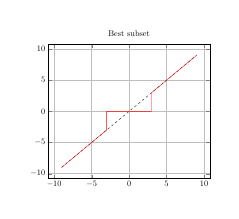
\begin{tikzpicture}[scale=0.3]
	\begin{axis}[title=Best subset, grid=major]
	\addplot[color=black, dashed] coordinates {
		(-9,-9)
		(9,9)
	};
	\addplot[color=red] coordinates {
		(-9,-9)
		(-3,-3)
		(-3,0)
		(3,0)
		(3,3)
		(9,9)
	};
	\end{axis}
	\end{tikzpicture}
    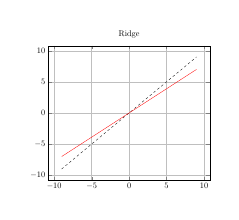
\begin{tikzpicture}[scale=0.3]
	\begin{axis}[title=Ridge, grid=major]
	\addplot[color=black, dashed] coordinates {
		(-9,-9)
		(9,9)
	};
	\addplot[color=red] coordinates {
		(-9,-7)
		(9,7)
	};
	\end{axis}
    \end{tikzpicture}
    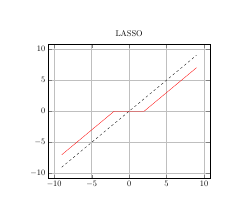
\begin{tikzpicture}[scale=0.3]
	\begin{axis}[title=LASSO, grid=major]
	\addplot[color=black, dashed] coordinates {
		(-9,-9)
		(9,9)
	};
	\addplot[color=red] coordinates {
		(-9,-7)
		(-2,0)
		(2,0)
		(9,7)
	};
	\end{axis}
    \end{tikzpicture}
        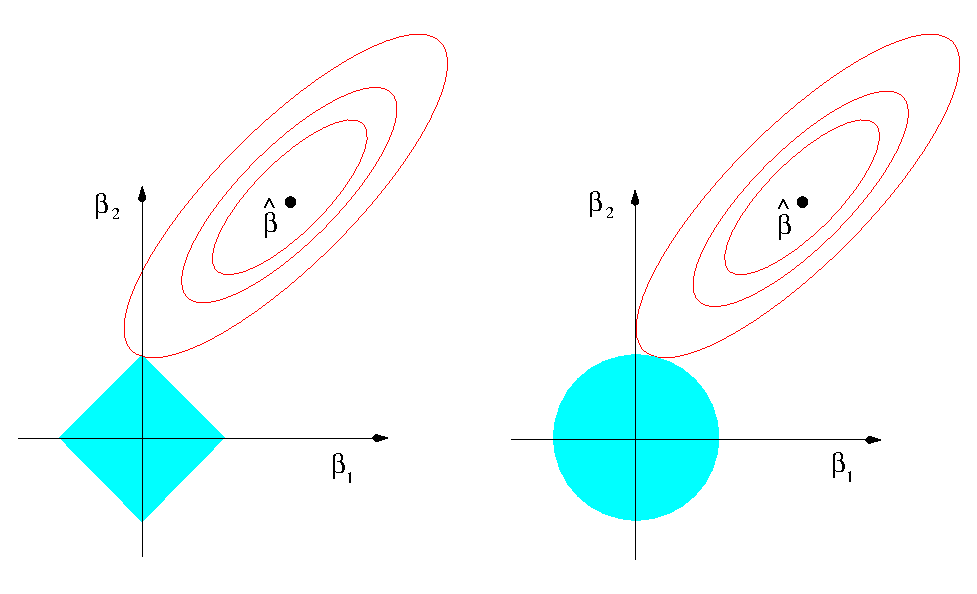
\includegraphics[width=0.3\textwidth]{figures/fig3-14.pdf}
    \end{figure}
\end{frame} 


\begin{frame}{Other variants of shrinkage methods}
    \begin{itemize}
        \item Elastic net penalty:
        \begin{eqnarray*}
            \lambda \left( \alpha \sum_{j=1}^p \beta_j^2+ (1-\alpha) \sum_{j=1}^p |\beta_j| \right)
        \end{eqnarray*}
        \item Least angle regression
    \end{itemize}
\end{frame}


\subsection{Derived input directions}

\begin{frame}{Derived input directions}
    \begin{itemize}
        \item General concept: transforms input $\vec{X}$ into a smaller subset of $\vec{z_m}$ and regress on $\vec{z_m}$
        \item Principal component regression:
        \begin{itemize}
            \item Transform non-orthonormal features into orthonormal directions using Principal Component Analysis (PCA).
            \item Choose $M$ directions that have the highest eigenvalues (explains the most variance) and discards the rest.
            \item Will revisit at a later lecture.
        \end{itemize}
    \end{itemize}
\end{frame} 


\begin{frame}{Partial Least Squares (PLS)}
    \begin{itemize}
        \item Algorithm:
        \begin{enumerate}
            \item Compute $\phi_{1i} = <\vec{x_j}, \vec{y}>$ for each $j$.
            \item First transformed direction $\vec{z_1} = \sum_j \phi_{1i} \vec{x_j}$, i.e., each direction is weighted by strength of effect on $\vec{y}$.
            \item Regress $\vec{y}$ on $\vec{z_1}$ to obtain $\theta_1$, orthogonalize $\vec{x_1}, ... \vec{x_p}$ wrt $\vec{z_1}$ via $x_j' = x_j - \frac{<\vec{z_1}, \vec{x_j}>}{<\vec{z_1}, \vec{z_1}>}\vec{z_1}$.
            \item Repeat until $M \leq p$ coefficients are obtained.
        \end{enumerate}
        \item Finds directions with high variance and high correlation with response.
    \end{itemize}
\end{frame} 


\begin{frame}{Bibliography}
    \bibliographystyle{plain}
    \bibliography{refs}
\end{frame}


\begin{frame}
    \Huge{\centerline{The End}}
\end{frame}

\end{document}

